\chapter{Pruebas durante el desarrollo y corrección de errores}
Una de las etapas más importantes durante el desarrollo de una aplicación es la de la creación y ejecución de pruebas. Desde ir probando determinadas configuraciones en la creación de formularios, comprobaciones de la navegabilidad e interacción de componentes hasta comprobar la fluidez y los tiempos de carga.
\\Antes de sacar un proyecto a producción han de pasar por un testeo y eso será lo que trataremos en este último capítulo.

\section{Pruebas durante el desarrollo}
Las herramientas que he utilizado durante el desarrollo del proyecto han sido tres:
\begin{itemize}
    \item \textbf{Postman}: Para poder realizar pruebas sobre la API.
    \item \textbf{Selenium}: Para poder realizar pruebas más que nada orientadas al envío de formularios.
    \item \textbf{Herramientas de Desarrollador de Google Chrome}: Para poder controlar la consola, algunos problemas de estilos y el envío y recibo de paquetes en la red.
\end{itemize}

\subsection{Postman}
Llevo utilizando Postman unos dos años y medio y me ha facilitado un montón las interacciones que me permite realizar con direcciones web.
\\Gracias a Postman he podido probar en este proyecto todas las interacciones que se pueden realizar con la API y el proxy que configuré en Angular.
\begin{figure}[h]
    \centering
    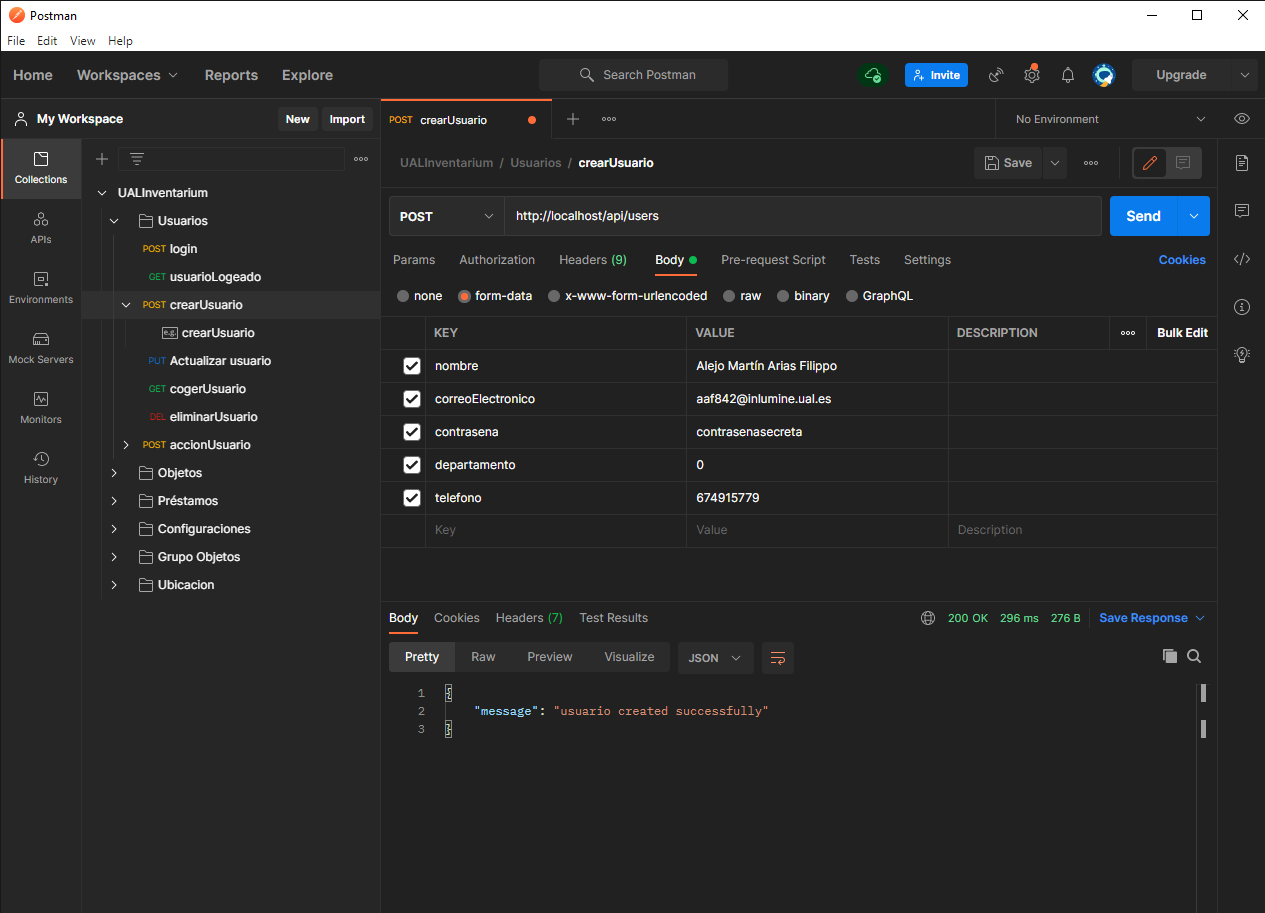
\includegraphics[scale=0.3,keepaspectratio]{../pruebas/postman_creation_user.png}
    \caption{Creando un usuario con Postman}\label{fig:postman-creation-user}
\end{figure}
Como podemos comprobar en la figura \ref{fig:postman-creation-user} hemos generado una solicitud POST para mandarla a la dirección \textit{/api/users} de nuestra página web. Que a su vez la redirigirá al registro probando el proxy.
\\Añadimos los parámetros dentro del campo \textit{Body} y al acceder a este dentro de \textit{form-data} que es la forma en la que hemos planificado el procesado de nuestras peticiones.
\\Luego de pulsar en el botón \textit{Send} podemos comprobar que se manda la solicitud porque nos llega una respuesta que hemos creado nosotros en la API, en este caso: \textit{`message': `usuario created successfully'}
\\Un punto bastante a favor que presenta Postman es que el conjunto de solicitudes que tengas se almacena en tu usuario por lo que al cambiar de dispositivo estas solicitudes se siguen manteniendo.
\\Otra herramienta que tenía incorporada esta aplicación y que he conocido hace poco es que tiene una herramienta que permite capturar solicitudes que salgan de un determinado puerto. Aparte de capturarlas, interpreta en su totalidad las estructuras de estas y podemos ver si hemos cometido algún fallo al mandar cualquier tipo del solicitud desde nuestra página.

\subsection{Selenium}
Gracias a la herramienta de grabación que aporta Selenium se han realizado bastantes pruebas en la página web.
\\Para poder utilizar la herramienta lo hemos hecho desde Google Chrome instalando la siguiente \href{https://chrome.google.com/webstore/detail/selenium-ide/mooikfkahbdckldjjndioackbalphokd}{\textbf{extensión}}.
\\Luego de instalarla abriremos la lista de complementos del navegador y seleccionaremos la aplicación. Pulsamos en crear nuevo proyecto y nos pide una \textit{url} para empezar a grabar unas pruebas. Ingresaremos la url \textit{http://localhost/register} para poder automatizar el proceso de registro.
\\Al empezar la grabación se nos abrirá una nueva ventana de Google Chrome y rellenaremos los datos como un proceso normal de registro pulsando finalmente en \textit{Registrarse}.
\\La prueba que se nos ha generado es la figura \ref{fig:registro-usuario-selenium}
\begin{figure}[h]
    \centering
    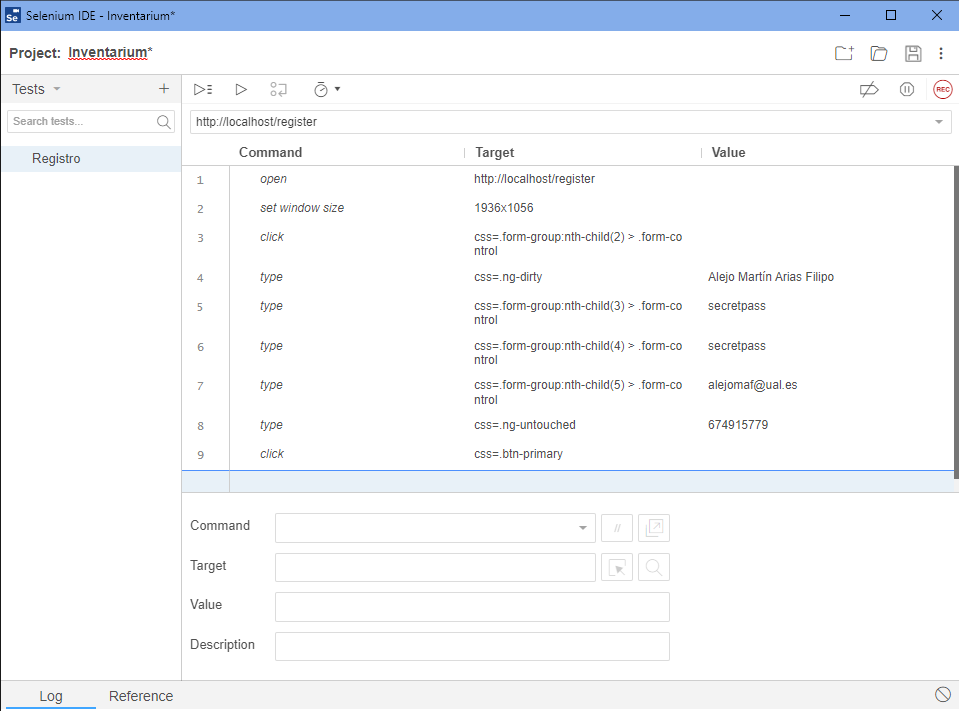
\includegraphics[scale=0.40,keepaspectratio]{../pruebas/registro_usuario_selenium.png}
    \caption{Registrando un usuario con Selenium}\label{fig:registro-usuario-selenium}
\end{figure}
\subsection{Herramientas de Desarrollador de Google Chrome}
Las Herramientas de Desarrollador de Google me ha acompañado en todas las fases del desarrollo de la aplicación. Desde las más tempranas hasta las más tardías.
\\El navegador Google Chrome brinda un conjunto de herramientas muy completo. Las tres que más he utilizado han sido:
\begin{itemize}
    \item \textbf{Elements}: Aquí podremos ver los elementos que tenemos en pantalla. Disponemos también de un inspector que nos permite pulsar sobre un elemento y localizarlo dentro de la estructura HTML que presenta el documento. También nos permite poder editar los estilos con los que estemos trabajando y ver los cambios en tiempo real. Estos no se aplican al documento pero ayudan en mucha medida a realizar arreglos de diseño.
    \item \textbf{Console}: Desde aquí podremos ver las salidas de consola que nos da la aplicación. En Angular para poder emitir señales en la consola utilizaremos \textit{console.log(``Objeto que queramos emitir'')}. Desde aquí podemos ver fallos que nos haya devuelto la aplicación y poder actuar en medida.
    \item \textbf{Network}: Esta sección la empecé a usar hace unos meses, nos ayuda en gran medida porque desde aquí podemos ver todos los paquetes entrantes y salientes desde el punto de vista del cliente.
\end{itemize}
\begin{figure}[h]
    \centering
    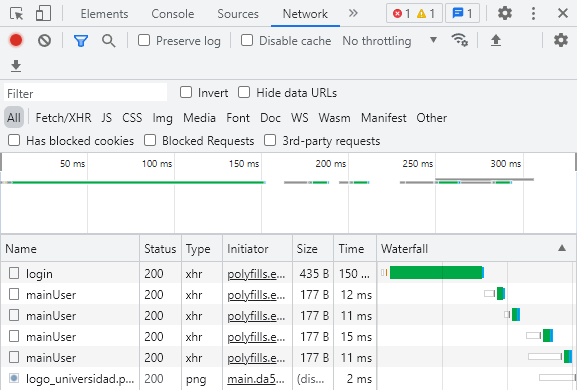
\includegraphics[scale=0.6,keepaspectratio]{../pruebas/network_dev_tools_chrome.png}
    \caption{Sección \textit{Network} dentro de las herramientas de desarrollador de Google Chrome}
\end{figure}
